\chapter{Analysis}
\section{The effects of the cuts}
How does the cuts imposed in the previous chapter affect the data then?
First we need to look at how the data looks, without any cuts. On \cref{fig:EENoCuts} the energy of the first \al-particle (E$_{\alpha1}$) is plotted against the energy of the second \al-particle (E$_{\alpha2}$).
This gives us a nice view of what is considered \al-particle pairs. There is a prominent line going diagonally through the graph, where both particles have approximately the same energy. This line is expected, as the \al-particles will have close to equal energy, when decaying from \ber. 

This means that there is a lot of particle pairs that have been identified as \al-\al, but probably was \al-noise, noise-noise, \al-\be\ or \be-\be\ pairs. 

The lines occurring from E$_{\alpha2} \approx \SI{400}{keV}$ are a clear example of a \al-\be\ pair. In this line, \al1 has been identified correctly as a \al-particle, which will have energies ranging from 500-\SI{6000}{keV}, whereas the the other particle has a more constant energy, corresponding to the energy a \be-particle can deposit in a detector. So by doing no cuts at all, we are left with a lot of cases where we have no real control over what particle type we are dealing with. 

\begin{figure}[H]
	\begin{subfigure}[t]{0.5\linewidth}
		\includegraphics[width=\linewidth]{../figures/EENoCuts.pdf}
		\caption{No cuts on the data}
		\label{fig:EENoCuts}
	\end{subfigure}
	\begin{subfigure}[t]{0.5\linewidth}
		\includegraphics[width=\linewidth]{../figures/EEAngleCut.pdf}
		\caption{An angular cut. The angle between the two partcles must be greater than $160\degree$.}
		\label{fig:EEAngleCut}
	\end{subfigure}
	\begin{subfigure}[t]{0.5\linewidth}
		\includegraphics[width=\linewidth]{../figures/EEMomentumCut.pdf}
		\caption{A momentum cut. The total momentum of the particles must be less than \SI{40}{MeV/c}}
		\label{fig:EEMomentumCut}
	\end{subfigure}
	\begin{subfigure}[t]{0.5\linewidth}
		\includegraphics[width=\linewidth]{../figures/EEBetaMulCut.pdf}
		\caption{A \be-multiplicity cut. There must exist at least one \be-particle and two \al-particles in the event. }
		\label{fig:EEBetaMulCut}
	\end{subfigure}
	\caption{A collection of the different effects the cuts impose on the energy of the \al-particles. On all the above figures, the energy of the first \al-particle (E$_{\alpha1}$) is plotted against the energy of the second \al-particle (E$_{\alpha2}$). The intensity scale is in logarithmic, to get a better view of all the different particle configurations.}
\end{figure}

\begin{figure}[H]
	\begin{subfigure}[t]{0.5\linewidth}
		\includegraphics[width=\linewidth]{../figures/EEMomentumCut.pdf}
		\caption{This cut shows only the momentum cut imposed on the data.}
	\end{subfigure}
	\begin{subfigure}[t]{0.5\linewidth}
		\includegraphics[width=\linewidth]{../figures/EEAngAndMoment.pdf}
		\caption{This cut shows the momentum \textit{and} the angular cut imposed on the data.}
	\end{subfigure}
\caption{A comparison of the momentum cut with and without the angular cut.}
\label{fig:AngAndMomentCompare}
\end{figure}

\subsection{The effect of the angular cut}
By imposing the angular cut, we get the first real reduction in data. If the angle between the two \al-particles are less than $\theta \approx 160\degree$, we sort away a good part of the \be-\al\ pairs, as seen on \cref{fig:EEAngleCut}. But there are still a good portion of wrong pairs left, and we move on to impose a cut on the momentum of the particles. 


\subsection{The effect of the momentum cut}
Again the aim is to sort the data, so that we can identify the particles. On \cref{fig:EEMomentumCut} the total momentum of the two particles has been limited to a maximum of \SI{40}{MeV/c}. This cut sorts away all of the vertical and horizontal lines from a \be-\al pair. With this drastic cut, it looks like there is no use for the angular cut, which might be true. On figure \ref{fig:AngAndMomentCompare} we can see the comparison of the effect of the momentum cut, with and without an angular cut. There does not seem to be a very large difference. Since momentum already takes the direction of the particles into account, as well as their energies, the angular cut will seem a bit redundant. However, we keep the angular cut on the data, as it will not take away any "good" measurements, but only some noise that slips through the multiplicity cut. Looking at \cref{fig:allCutsCompare}, we see the blue line as the momentum cut and the magenta line as the momentum and angular cut. The two histograms lie very close to each other, except in the low energy ranger. Here we see a slight reduction in the magenta line, indicating that the pure angular cut will sort some \be-particles from the data. It is therefor a justified cut to still impose on the data. 
 


\subsection{The effect of the multiplicity cut}
The multiplicity of the \be-particles should not interfere so much with the \al-particles, but looking at \cref{fig:EEBetaMulCut}, we see a drastic change in the pairs with energies far from each other. This is due to a general reduction in data. With the requirement that there must be one \be-particle present in the event \textit{and} that it must have hit either Det2 or DetD, we are left with a lot fewer measurements, which in turn gives a lower probability of noisy pairs. 

\subsection{The combined effect of all the cuts}
By combining all of the cuts we are satisfied with the sorting of particles. 
On \cref{fig:EEAllCuts} we see the effect of all the cuts.
There is a very prominent line of particles with roughly the same energy. 
The line is thinner at higher energies, and widens as it goes towards lower energies. 
The reason for the widening, is the recoil energy from the \be-decay.
If the \al-particles have low energy, they are more susceptible to other forces around it, and will lose a larger portion of their energy to the \be-particle recoil. \\
\begin{figure}[h]
	\centering
	\includegraphics[width=\linewidth]{../figures/cutCompare.pdf}
	\caption{A comparison of all the cuts, with the energy of one \al-particle shown. }
	\label{fig:allCutsCompare}
\end{figure}
\begin{figure}[h]
	\centering
	\includegraphics[width=\linewidth]{../figures/EE.pdf}
	\caption{The energy of the first \al-particle plotted against the energy of the second \al-particle. All of the data reduction cuts are used here.}
	\label{fig:EEAllCuts}
\end{figure}
On \cref{fig:allCutsCompare} all the cuts are shown as individual histograms, highlighting the effect that each cut provides. Here it is worth noting that not all \be-particles have been successfully removed from the data. A slight peak at low energies still remain for the black line in the figure. This is also clear on \cref{fig:EEAllCuts}, where the there is a high intensity at the $\approx$ \SI{200}{keV} energy range. 

An interesting effect that can be seen on the data, is the importance of the momentum cut. Looking the red and green line, we see a soft reduction in counts, different from the more rapid fall around \SI{6}{MeV} for the magenta line. This is because there can be events where a particle will hit the detector, triggering it to measure, and before it turns completely off for detecting, another particle hits, and some of the the energies from both particles are measured as one particle. 
So the momentum cut will also cut bad detection events away from the data in the high energy regime. 



So far we have considered that only the \al-particles are sorted correctly. But there is still a question about whether the \be-particles will be clouded by wrong identifications. 
On \cref{fig:beSpectrum} we see the energy deposited in the two detectors that are capable of measuring \be-particles, and the pad behind Det2.
The energy from the pad and DetD, shows one peak around \SI{400}{keV} and \SI{300}{keV}, respectively. 
Det2 shows two peaks, one close to \SI{400}{keV}, and one close to \SI{800}{keV}. This is rather interesting, as we do not expect \be-particles to deposit two different energies. Both detectors and the pad where \SI{1000}{\mu m} thick, so we expect that the energy deposited would be roughly the same. The stopping power of silicon predicts an electron will deposit around \SI{300}{keV} - \SI{500}{keV} in \SI{1000}{\mu m} silicon \cite{NIST_ASD}, depending on the actual energy of the \be-particle. So the first peak of the blue line is most likely the "real" \be-energy. 
An explanation as to why we see the secondary peak, could be that this detector was part of the trigger system, that detects when a particle has been hit anywhere in the setup. There is a lower bound on what energies that can trigger the system, and it is placed at \SI{500}{keV}. 
So this peak most likely stems from false detection caused by the triggering, since DetD was not part of the trigger, and did not produce two peaks.

\begin{figure}[h]
	\centering
	\includegraphics[width=\linewidth]{../figures/betaSpec.pdf}
	\caption{Energy deposited by \be-particles in Det2 (blue), DetD (red) and Pad2 (green). PadD has been omitted, due to an error in the pad.}
	\label{fig:beSpectrum}
\end{figure}

\section{The excitation energy of $^8$Be}
With the \al-particles sorted correctly, we can start to look at the excitation energy of \ber. As mentioned in \cref{sec:beta} the \be-decay of \li will populate a broad exited state of \ber. This will give a more wide peak than we normally see in \al-decays. On \cref{fig:bata} the energy sum of the \al-particles has been plotted as the blue line. The peak lies closely to the mean energy of the exited state of \SI{3.03}{MeV}, and then has a long tail all the way up to the around \SI{16}{MeV}.
\begin{figure}[h]
	\centering
	\includegraphics[width=\linewidth]{../figures/bataraCompare.pdf}
	\caption{A comparison between the spectra of the excited state in \ber from this experiment(blue), and a fit found by Bhattacharya \cite{bata} (green).}
	\label{fig:bata}
\end{figure}
At the low end of the spectra, there is a small peak just before the beginning of the main peak. This is the reminiscence of low energy \be-\be\ pairs that have not been sorted in the data. We will not worry too much about this, as the interesting properties of the spectra lies at higher energies than the main peak.

The green line is a fit made to another experiment by Bhattacharya \cite{bata}. The fitted green line has been scaled accordingly,for a better comparison between the two plots. 
The plots differ a lot in the low energy range, as the \be-particle contribution is rather prominent. But around the peak and at higher energy, the fit and our data follows nicely. At the very end, they differ again, as there seem to be some noise in our data, since the counts are too low to be considered otherwise. 

\subsection{Lepton recoil}
E. K. Warburton \cite{PhysRevC.33.303} argues that the lepton recoil will be significantly small, and can be neglected, when observing the exitation spectra of \ber. This means that measuring one \al-particle and multiplying the energy with 2, will be just as good a measurement as measuring both, and adding their energies. 
As Bhattacharya finds \cite{Bhattacharya:2002gc}, it cannot be neglected, and as we have shown in \cref{fig:recoil} and \cref{fig:recoilGauss}, the leptons will have a noticeable impact on the excitation of \ber, as it seems that the red line peaks at lower energies than the blue. The fit on \cref{fig:beSpectrum} from \cite{bata} also takes this effect into account. 


\begin{figure}[h]
	\begin{subfigure}[t]{.48\linewidth}
		
		\includegraphics[width=\textwidth]{../figures/recoil.pdf}
		\caption{Difference between twice the energy of one \al-particle and the sum of two \al-particles. The red line indicates the sum of both \al-particles in coincidence. The blue line shows the double energy of a single \al-particle.}
		\label{fig:recoil}
	\end{subfigure}\hfill
	\begin{subfigure}[t]{.48\textwidth}
		
		\includegraphics[width=\linewidth]{../figures/recoilGauss.pdf}
		\caption{A plot of the difference in energy in the range \SI{2}{MeV} to \SI{4}{MeV}. The recoil of the leptons will have a notable difference in energies in this range.}
		\label{fig:recoilGauss}
	\end{subfigure}
	\caption{}
\end{figure}

\section{Angular efficiency of the setup}
Since the detectors are unable to cover the entire solid angle, there will always be some mutual angles that are more likely to be measured. 
If we only look at one detector, a very large number of angles are not covered, but small mutual angles such as $\theta \approx 0$, are very easy to measure, as it is just a measurement of two particles in the same pixel. 
This effect becomes apparent on \cref{fig:oneDetEff}, where the angular efficiency is shown for Det2. For a single detector, there cannot be angles of $\theta = 90$ and higher, as the detector is flat. In this detector, the lowest angle found was $\theta = 77\degree$.\\

\begin{figure}[h]
	\includegraphics[width=\linewidth]{../figures/det2Eff.pdf}
	\caption{The angular efficiency of a single detector (Det2). For one flat detector, there can never be angles of $90\degree$ and higher. An efficiency has been multiplied to the histogram, which is why the y-axis is a bit arbitrary.}
	\label{fig:oneDetEff}
\end{figure}
In this setup however, we have a cube of square detectors, who's normal vectors are all pointing in towards target at the center. This gives a much larger coverage of all mutual angles. 
The placement of the detectors gives that angles around $\theta \approx 90 \degree$ are also very favored. This makes sense, almost no matter what pixel was hit, there is a corresponding pixel $90\degree$ to both sides, up and down. In the same way, will there always be a corresponding pixel $\approx 180\degree$ from each pixels. This effect can be seen on \cref{fig:effAllDet}. \\
This histogram was created using the spacial coordinates of each pixel in the setup. A list of all pixel positions was gathered. The mutual angle between every pixel was found, that is $(16\cdot 16 \cdot 6)^2 =$ \num[group-separator={,}]{2359296} possible angles in the setup. 


\begin{figure}[h]
	\includegraphics[width=\linewidth]{../figures/allDetEff.pdf}
	\caption{Two normalized histograms of the angular efficiency of the entire setup. The red histogram does not account for the effective area of a pixel. The blue is the true angular efficiency.}
	\label{fig:effAllDet}
\end{figure}
There is still a geometric effect that is not accounted for in the above analysis. We need to consider that not all pixels in the detector has the same effective area. 
The pixel furthest out in a detector will have a effective area smaller than the area of a pixel in the center. This effect can be seen on \cref{fig:MexiHatDetector}. Here we see that there is a much higher count of particles hitting the center of the detector, and fewer hitting the edges. A white line crossing through the middle is a defect strip, which did not measure anything. Sadly, some of the detectors had defect strips, which skews the effective angle and the measured. 
\begin{figure}[h]
	\begin{subfigure}[t]{.5\linewidth}
		\centering
		\includegraphics[width=\linewidth]{../figures/mexihatDet2.pdf}
		\caption{A plot over the number of hits in each strip for Det2. The white line in the middle is a defect strip, that did not measure anything.}
		\label{fig:MexiHatDetector}
	\end{subfigure}
	\begin{subfigure}[t]{.5\linewidth}
		\centering
		\includegraphics[width=\linewidth]{../figures/mexihatDet2THEORY.pdf}
		\caption{A theoretical intensity Det2. }
		\label{fig:MexiHatDetectorTheory}
	\end{subfigure}
\caption{}
\end{figure}

To account for the geometric effects of the detectors, each pixel will be associated with a corresponding area-efficiency $(\text{Eff}_A)$.
This is calculated as 
\begin{equation}
\text{Eff}_A = \dfrac{A\cos(\theta) }{ 4 \pi r^2},
\label{eq:eff}
\end{equation}
where $r$ is the distance to the pixel, $A$ is the area of the pixel and $\theta$ is the angle between the hit direction and the normal vector of the detector as shown on \cref{fig:EffGeometry}. As the angle becomes greater, the effective area of the pixel decreases. 
The area of all pixels are the same for all detectors, so the constants $A$ and $4\pi$ can be ignored when comparing the efficiency. 


\begin{figure}[h]
	\centering
	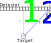
\includegraphics[width=.7\linewidth]{../figures/detektorEffDrawingv2.pdf}
	\caption{An illustration of two hits in different pixels. The blue hit will see a smaller effective area of the pixel by a factor determined by \cref{eq:eff}, as the projection of the blue line onto the dashed line decreases as $\theta$ increases.}
	\label{fig:EffGeometry}
\end{figure}

On \cref{fig:effAllDet} two histograms can be seen. The red line represents the angular efficiency of the setup, without accounting for the relative area of the pixels, while the blue line is a weighted histogram for the same angles, with each pixels relative area accounted for. \\
The form of the two histograms are quite similar around 1, 0 and $-1$ but in between there is a rather prominent difference. Therefore it is important that the effective area of the pixel is accounted for, when we in \cref{sec:betaAngle} will look at the angular correlations of the \be-particle in the setup. 



\section{Angular correlations of \be-\al\ particles}
\label{sec:betaAngle}
From what we know from \cite{isotrop} the \be-particles must have an isotropic distribution to the \al-particles. 
This is done by first finding the angle between the first \al-particle \al$_1$ and the \be-particle, and create a histogram of this. Then the angle between the second \al-particle \al$_2$ and the same \be-particle is measured, and a histogram is created. The two histograms are then added, to get the full picture of the mutual angles of the particles. 
This can be seen on \cref{fig:effwithweight} as the green line.  

The blue line in this figure is the angular efficiency for the specific case, where the \al-particles can hit in any given detector, but the \be-particles can only hit in the two specific detectors Det2 and DetD. The two histograms has both been normalized, for a better comparison. By dividing the two histograms with each other, we get a better comparison. If they where to be close to equal, we would see a flat curve. But what we see on \cref{fig:dataDivEff} is not very flat. 
There are small fluctuations in the line, which stems from the inaccuracy of calculated angular efficiency. But the main shape of the curve is at most time not constant.

\begin{figure}[h]
	\centering
	\includegraphics[width=\linewidth]{../figures/betaAngles/betaAngle.pdf}
	\caption{The measured \be-\al\ angular correlation is shown as the green line. The blue line shows the angular efficiency of the setup. Both histograms has been normalized, for a better comparison.}
	\label{fig:effwithweight}
\end{figure}

\begin{figure}[h]
	\centering
	\includegraphics[width=\linewidth]{../figures/betaAngles/dataDivEff.pdf}
	\caption{Data divided by the angular efficiency. }
	\label{fig:dataDivEff}
\end{figure}

There are two different explanations as to why this might be.
The first explanation is that the beam did not hit the target in the center. The calculated efficiency assumes that the beam hits precisely in the middle, but in any setup, there can be a few millimeters of errors. 

By finding the angular efficiency of the setup, with different values for the center and comparing this to the measured angles, we have found a slight correction for the center of the beam. This can be seen on \cref{fig:centerCorrection}, where the beam has been moved to the coordinates $(-3, -3, 0)$, as opposed to the previous of $(0, 0, 0)$. The division fo the two histograms on \cref{fig:dataDivEffCenter} shows a more stable line from $\cos(\theta)= -0.4$ to $\cos(\theta) = 0.4$, but the edges are still not very alike. Looking at $\cos(\theta) = 1$, we see a rapid fall, which indicates that we have measured a lot fewer parallel \be\ and \al-particles than the setup is designed to handle. 
This can be due to the fact that some of the strips where defect. The calculated angular efficiency does not know which strips where defect, and and will therefore have a lot higher efficiency for parallel particles. The defect strips will therefore also play a role in the grand scheme, and is a possible explanation as to why there is a difference in the calculated and the measured data. \\
Another effect that will sway the data, is the target holder. This device will provide a shadow over the top and bottom detector, and since one of the \be-detectors are the bottom one, it will skew the data in a unforeseeable way. An example of this can be seen on \ref{fig:mexihatDet4}, where the shadow can be seen going from $(0,0)$ to $(16,16)$. This detector also has two dead strips, which is the white lines.  
\begin{figure}[h]
	\begin{subfigure}[t]{.48\linewidth}
		\centering
		\includegraphics[width=\linewidth]{../figures/betaAngles/centerCorrectedAndData.pdf}
		\caption{The angular efficiency and the data, with a correction for the center of the beam. }
		\label{fig:centerCorrection}
	\end{subfigure}\hfill
	\begin{subfigure}[t]{.48\linewidth}
		\centering
		\includegraphics[width=\linewidth]{../figures/betaAngles/dataDivEffCenterCorrected.pdf}
		\caption{Measured \be-\al-particle angular distribution divided by the calculated angular efficiency of the setup, with a correction for position of the beam. }
		\label{fig:dataDivEffCenter}
	\end{subfigure}
\caption{}
\end{figure}

\begin{figure}[h]
	\centering
	\includegraphics[width=.7\linewidth]{../figures/mexihatDet4.pdf}
	\caption{A plot over the number of hits in Det4. A shadow from the target holder is visible as a diagonal from $(0,0)$ to $(16,16)$.}
	\label{fig:mexihatDet4}
\end{figure}


